\chapter{Fortschreitende Elektronikentwicklung}\label{cha:Elektronikentwicklung}

In diesem Kapitel der Arbeit wird die Umsetzung der diversen Konzept und Strukturanforderungen in Hardware betrachtet. Dabei werden hier ausgesuchte Beispiele aus mehreren Vergangenen Jahren Vorgestellt und Technisch erläutert.
Dabei wird die kontinuierlich Fortschreitende Implementierung von Erfahrung im Zusammenspiel mit dem Modularen Gesamtkonzept aufgezeigt.

\section{Ursprünglicher Elektronikzustand}

Die in der Saison 2014 begonnen Voruntersuchungen fanden mit dem Flugsystem "Maya" statt.
Abseits von Strukturellen und Flugmechanischen Problemen war auch die Elektronik eine kontinuierliche Quelle von Fehlern und Ausfällen des Flugzeugs.
Dies war größtenteils auf die Mangelnde Erfahrung im Umgang mit einem System eines solchen Komplexitätgrades zurückzuführen.Aber auch eine noch unzureichende Ausstattung mit Werkzeug und Testmöglichkeiten und Methoden in Kombination mit der Unübersichtlichen Kabelführung erschwerte die Fehlersuche.

-->> Hier Bild mit Kabelsalat in der Maya

\section{Neue Platinenaufteilung}

Aus diesen Erfahrungen entstand das Eingangs vorgestellte Konzept für die Elektronik des Fliegers.
Dieses Konzept wurde 2015 erstmals angewandt, um eine Übersichtliche und einfach handhabbare Hardwareplattform mit leicht überprüfbaren Funktionen Umzusetzen.

\subsection{Leistungsplatine}

\subsubsection{Schaltplan}

\begin{figure}[H]
\centering
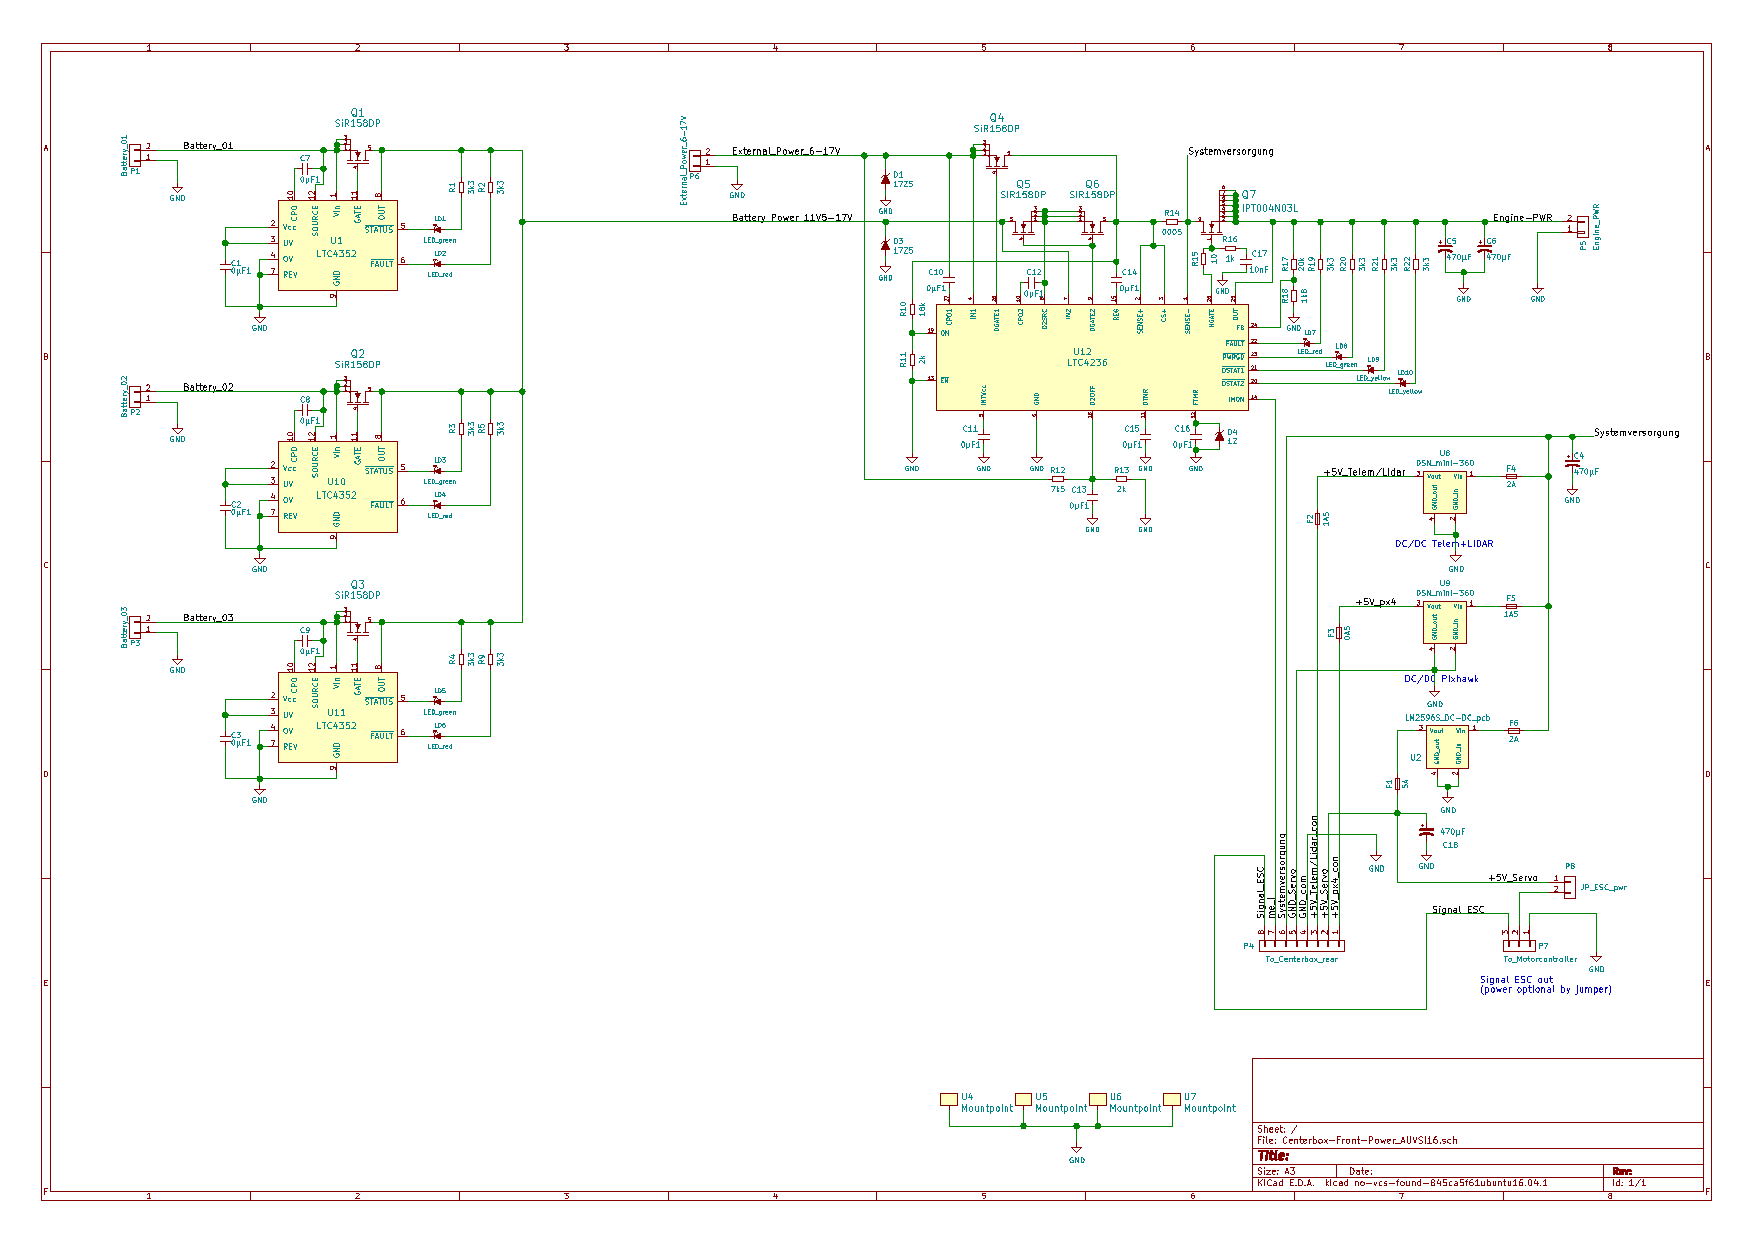
\includegraphics[width=0.9\textwidth]{bilder/Centerbox-Front-Power_AUVSI16.pdf} 
\caption{Schaltplan der Leistungsplatine} 
\label{fig:Schaltplan der Leistungsplatine}
\end{figure}

\subsubsection{Platinenlayout}

\subsection{Autopilotenplatine}

\subsubsection{Schaltplan}

\subsubsection{Platinenlayout}

\section{Bedien- und Schutz Konzepte}

\subsection{Eineindeutige Verbinderauswahl}

Für die angepasste Führung von Leistungspfaden und Signalpfaden wurden im Laufe des bisherigen Projekts je zwei verschiedene Steckersysteme eingesetzt.

Die Hochstromverbindungen werden stets mit Kabelquerschnitten von 1,5 mm ausgeführt. Der Mantel besteht aus PVC außer in der Nähe von heißen Bauteilen an denen Silikon zum einsatz kommt.
Zu beginn wurden als Hochstromstecker Bauteile vom Typ BLAAA der Firma BLuuub verwendet.
Diese wurden von den meisten Zukaufbaugruppen der Pixhawk Systems verwendet und ermöglichten eine mechanisch kodierte eindeutige Verbindung.
Sie sind für Ströme von Blaaa Ampere und Spannungen von FUUUU freigegeben.
Jeoch waren diese Steckverbinder nur zur Lötmontage vorgesehen. Es wurde die Erfahrung gemacht das die Verbindungen zur Kabelseite immer wieder versagten. Teils wegen Qualitativ ungenügender Lötstellen, teils wegen Brüchen durch Handhabung mit Bewegung des Kabels am Übergang von der Lötstelle zum Kupferkabel am Steifigkeitssprung.

-->> Bild von T90 und Powepol 55 

Daraufhin wurde ein neues System mit Crimpmontage gesucht.
Hierfür wurde das System Powerpol der Firma FUUU ausgewählt. Die Steckverbinder sind bis zu einem Dauerstrom von 55 Ampere und einer Spannung von 300 V freigegeben.
Die Kabelbrüche wurden mit dem Crimpsystem als Fehlerquelle behoben. Sie können in den Quadratischen Gehäusen beliebig nebeneinander eingeclipt werden was größere Steckblöcke ermöglicht. Jedoch führte diese variable Montierbarkeit auch immer wieder zu wiedersprüchlicher Montage von Ladekabeln und Akkus bezüglich der Polposition.
Außer einer klaren Standardisierung der Polung wurde bisher noch keine Konzept gefunden Bedienfehler auszuschließen. 



<<<<< Hier noch Signalstecker  Lumberg MSF1 und JST PA


\subsection{Priorisierung externer Anschlüsse im Ground Handling}

Die Priorisierung bestimmter Energiequellen wurde erstmals in der Saison 2016 eingesetzt.
Damit wurde es möglich, an einen Flugfertig Montierten System alle Vorflugkontrollen und die Kalibrierung der Autopilotensysteme durchzuführen ohne die Missionsenergieversorgung zu entladen. Dazu wurde ein ähnlicher Akku mit ebenfalls vier Zellen an einem Zentralen Anschluss in der sogenannten WingCenterBox Verbunden. Solange dieser Angeschlossen war wurde sämtliche Energie für die Steuerelektronik, die Servosysteme und die Motortesläufe ausschließlich aus diesem bezogen. Die zentrale Unterbringung des Anschlusspunktes in der WingCenterBox stellte sicher das ein Schließen der Box Abdeckung nur nach vorheriger Demontage des externen Akkus möglich war, was Bedienungsfehler ausschloss.

--> Bild 2016

-->>Schaltplan 2016 


\subsection{Schutz vor Fehlbedienung im Leistungspfad}

\subsubsection{Die Ideale Diode}

\subsubsection{Die Ideale Diode als Modul}

\subsubsection{Optimierung der Idealen Diode}

\section{Integration von Zukaufbaugruppen}

\section{Mechanische Integration im Flugsystem}